\section{Model with incomplete information}
An interesting scenario to model is when the nodes lack information about the other nodes type. The way we model this is by letting nature selecting whether a player is insured or not, a node is insured with probability $p$, and not insured with probability $1-p$. 
All nodes know their own type, but in the link establishment process there are only one node who knows the type of the other. The other node only know the probability of the other node being insured or not. 
What we want to find is if it possible for the nodes with incomplete information to distinguish a insured node from a non-insured one. In order to form insurable topologies although we have a scenario with incomplete information. 
\subsection{Analyzis}
When facing a game like this, there exists two types of equilibriums, one where node 2 is able to seperate node 1's type, seperating equilibrium. The another where he can seperate them, pooling equilibrium. 
In this game we have two types of node, type 1 $(t1)$: insured and type 2 $(t2)$: not insured. 
\subparagraph{Node 2 is insured}
Since every node knows their own type, there are two different games to model, one where node 2 is insured, and the other where he is not insured. We start with the one where he is insured.
Node 1's type is chosen randomly by nature, with probability $p$ of being type 1 and $1-p$ of being type 2.
\begin{figure}[h]
\centering
  \centering
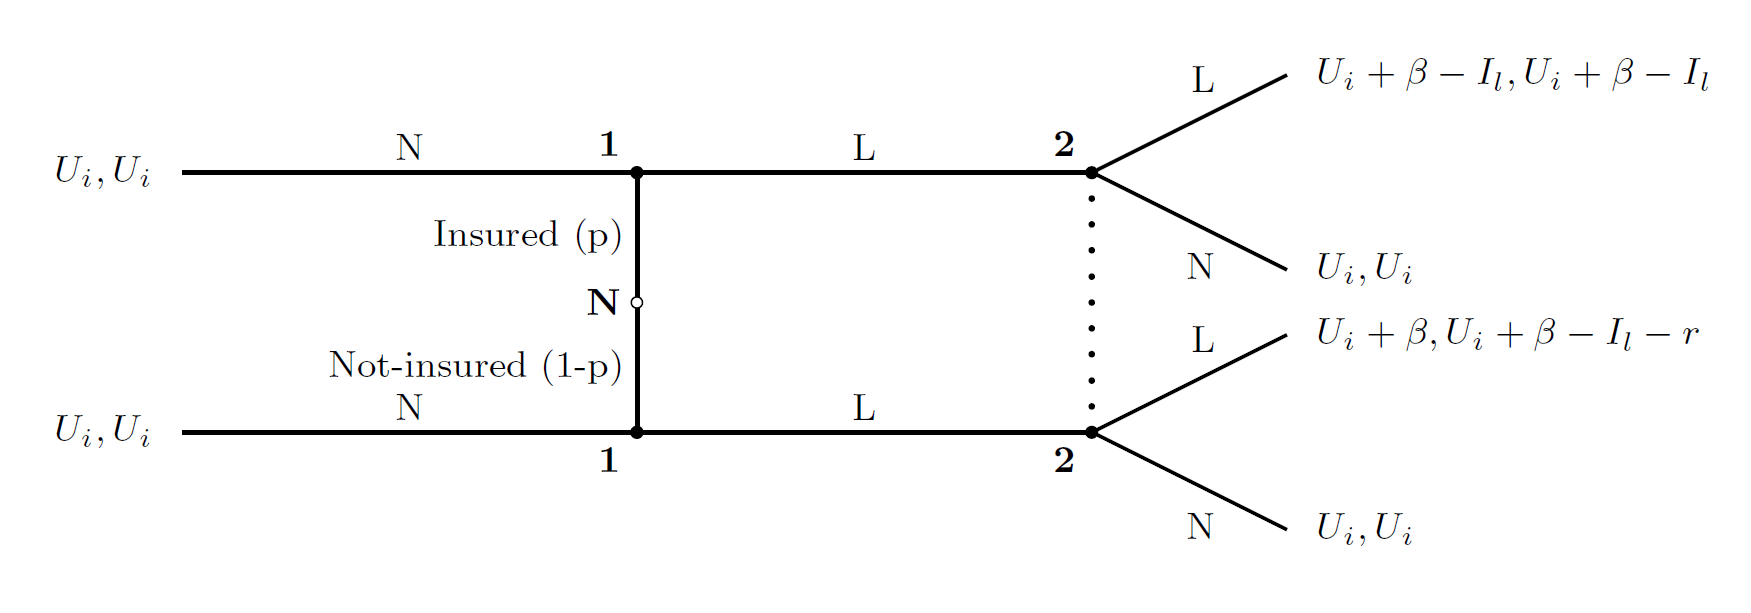
\includegraphics[width=1\linewidth]{../Figures/SignalingGameInsured.png}

\caption{Signalling game with two nodes, node 1's type choosen by nature, node 2 is insured. Node 1 have complete information, node 2 suffer from incomplete information, and act on best response functions based on beliefs. \label{fig:signalingInsured}}

\end{figure}

In the extensive-form shown in Figure \ref{fig:signalingInsured}, we see that $t2's$ strategy L dominates N, and thus $t2$ will never play $N$.
\subparagraph{Separating equilibrium}
Since node 1 will never play $N$ as type 2, there are only one possible separating equlibrium, type 1 plays $L$ and type 2 plays $N$. Hence node 2's beliefs are as in Eq.(\ref{eq:node2belief}).
\begin{equation}
    \sigma_{1}(t_{i})= 
\begin{cases}
   N,& \text{if } t1\\
   L,& \text{if } t2  
\end{cases}
\label{eq:node2belief}
\end{equation}
Let $\mu_{1}(t_{i} | N )$, denote the probability that node 1 is of type $t_{i}$. By using bayes rule we get this equation:
\begin{equation}
\mu_{1}(t_{1} | N )=\frac{P(N|t_{1})P(t_{1})}{P(N)}=\frac{P(N|t_{1})P(t_{1})}{P(N|t_{1})P(t_{1})+P(N|t_{2})P(t_{2})}
\end{equation}

With node 2's belief, we get that $\mu_{1}(t_{1} | N )=1$ and $\mu_{1}(t_{2} | L )= 1 $. We can now calculate node 2's expected utility from playing L and N:
\begin{eqnarray}
EU_{2}(L,L)=\mu_{1}(t_{1} | L )U_{2}(L,L;t_{1})+\mu_{1}(t_{2} | L )U_{2}(L,L;t_{2}) \nonumber\\
\llap{$\rightarrow$\hspace{50pt}}EU_{2}(L,L)=U_{i}+\beta-I_{l}-r \\
EU_{2}(N,L)=\mu_{1}(t_{1} | L )U_{2}(N,L;t_{1})+\mu_{1}(t_{2} | L )U_{2}(N,L;t_{2})\nonumber\\
\llap{$\rightarrow$\hspace{50pt}}EU_{2}(N,L)=U_{i}
\end{eqnarray}
From these two equations we see that the best response of node 2($BR_2$) when he observes the other node choosing action $L$ is:
\begin{equation}
BR_{2}(L)=
\begin{cases}
L, & \text{if }\beta - r \geq I_{l}\\
N, & \text{if } \beta -r<I_{l}
\end{cases}
\label{eq:insuredBR}
\end{equation}
Node 2's expected utility when type 1 chooses N, is easily seen to be $U_{i}$. 
To confirm if this is a separating equilibrium we must see if node 1 has any incentive to deviate from the strategies in node 2's belief.
Type 2 will never deviate, so lets investigate type 1.
In order to get node 1 to be willing to play N when he knows node 2's best response function, the following must hold: $\beta<I_{l}$. If this is true, then node 2's best response is to play N. I.e. the only separating equilibrium is the following:

\begin{eqnarray}
\beta<I_{l}\\
 \sigma_{1}= 
\begin{cases}
   N,& \text{if } t1\\
   L,& \text{if } t2  
\end{cases}\\
BR_{2}(\sigma_{1})=N
\end{eqnarray} 
This means that in a separating equilibrium, the game will end up with no link establishment.
\subparagraph{Pooling equilibrium}
In a pooling equilibrium node 2 will not be able to distinguish the two types, and since $t1$'s strategy $L$ dominates $N$, i.e. there is only one possible equilibrium, the one where both types of node 1 plays $L$.
\begin{equation}
    \sigma_{1}(t_{i})= 
\begin{cases}
   L,& \text{if } t1\\
   L,& \text{if } t2  
\end{cases}
\label{eq:node2beliefpooling}
\end{equation}
By using bayes rule we get that $\mu(t_{1}|L)=p$ and $\mu(t_{2}|L)=1-p$.
Node 2's expected utility is then:
\begin{eqnarray}
EU_{2}(L,L)=p(U_{i}+\beta-I_{l})+(1-p)(U_{i}+\beta-I_{l}-r)\nonumber\\
\llap{$\rightarrow$\hspace{50pt}}EU_{2}(L,L)=U_{i}+\beta-I_{l}-r+pr\\
EU_{2}(N,L)=U_{i}
\end{eqnarray}
From this we get node2's best response:
\begin{equation}
BR_{2}(L)=
\begin{cases}
L ,& \text{if } \beta + rp-r\geq I_{l} \\
N ,& \text{if } \beta +rp -r < I_{l} 
\end{cases}
\end{equation}
By using this best response function, node 1 sees that as long as $\beta>I_{l}$ he will never deviate from node 2's beliefs. And it is a pooling equilibrium where both nodes choose $L$, as long as $\beta>I_{l}$ and $\beta +rp-r>I_{l}$.
We also know that: $rp-r\leq0$ is allways true, and thus there also exists a pooling equilibrium where node 1, plays $L$, and node 2, plays $N$. This equilibrium will occur when $\beta>I_{l}$ and $\beta+rp-r<I_{l}$.
\subparagraph{Node 2 not insured}
Here we will analyze the game when node 2 is not insured.
The rules of the game are as before, the only thing that has changed is the type of node 2, and thus the payoffs are different and we need to see if there exists separating and pooling equilibrium in this game as well.
\begin{figure}[h]
\centering

  \centering
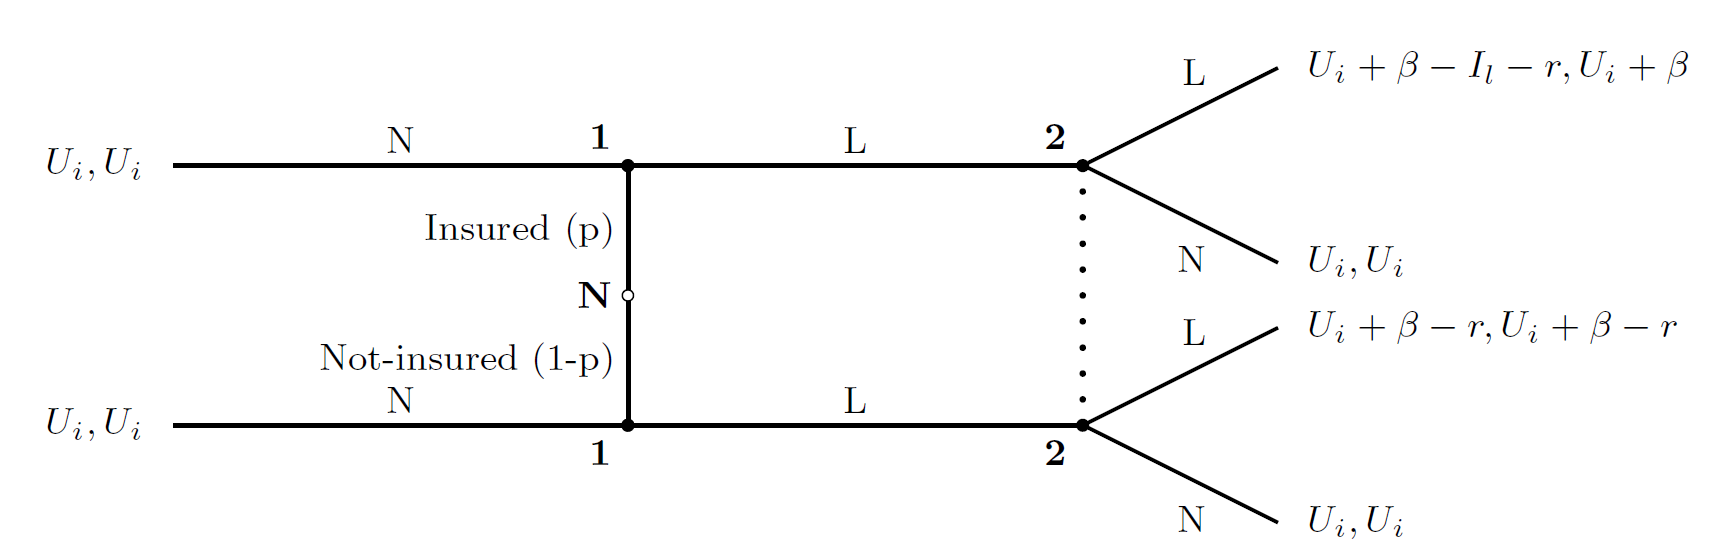
\includegraphics[width=1\linewidth]{../Figures/SignalingGameNotInsured.png}

\caption{Signalling game with two nodes, node 1's type choosen by nature, node2 is not insured. Node 1 have complete information, node 2 suffer from incomplete information, and act on best response functions based on beliefs. \label{fig:signalingNotInsured}}

\end{figure}
\subparagraph{Separating equilibrium}
In this game there is no dominant strategy for node 1, thus we have to check for the two possible separating equilibriums.
We start with the separating equilibrium with the beliefs shown in Eq.(\ref{eq:node2beliefnotinsured}).
\begin{equation}
    \sigma_{1}(t_{i})= 
\begin{cases}
   L,& \text{if } t1\\
   N,& \text{if } t2  
\end{cases}
\label{eq:node2beliefnotinsured}
\end{equation}
With the beliefs in Eq.(\ref{eq:node2beliefnotinsured}), this is node 2's expected payoffs:
\begin{eqnarray}
EU_{2}(L,L)=(U_{i}+\beta) \\
EU_{2}(N,L)=(U_{i})
\end{eqnarray}
From this we see that his best response when node 1's action is L, is to allways play $L$: \begin{equation}
BR_{2}(L)= L
\end{equation}
To see if this is an equilibrium, we have to see if node 1 has any incentive to deviate. 
We need to check for the two types of node 1:
If $\beta>r$ then type 2 would deviate, because he could achieve a higher payoff by playing $L$, given the beliefs of node 2 in Eq.(\ref{eq:node2beliefnotinsured}). So we know that for this to be an equilibrium, \begin{equation}
\beta < r
\label{eq:sepcondition}
\end{equation}  
When analyzing from node 1 type 1's perspective, for him to play L, this has to hold: $U_{i}+\beta-I_{l}-r > U_{i}$. The only way this can hold is if $\beta>I_{l}+r$. We see that Eq.(\ref{eq:sepcondition}) is violating this condition, and thus we have no separating equilibrium with the beliefs in Eq.(\ref{eq:node2beliefnotinsured}).

Now lets look at the other possible separating equilibrium, see Eq.(\ref{eq:node2beliefnotinsured2}).
\begin{equation}
    \sigma_{1}(t_{i})= 
\begin{cases}
   N,& \text{if } t1\\
   L,& \text{if } t2  
\end{cases}
\label{eq:node2beliefnotinsured2}
\end{equation}
Node 2's expected payoffs are as follows:
\begin{eqnarray}
EU_{2}(L,L)=U_{i}+\beta-r \\
EU_{2}(N,L)=U_{i}
\end{eqnarray}
From this we get the best response function:
\begin{equation}
BR_{2}(L)=
\begin{cases}
L ,& \text{if } \beta\geq r \\
N ,& \text{if } \beta<r 
\end{cases}
\end{equation}
For this to be a separating equilibrium, we need to see if node 1 would deviate from node 2's beliefs. 
Type $t1$ will not deviate as long as $\beta<I_{l}+r$. Type $t2$ will not deviate if $\beta \geq r$, if this condition is true, we see that node 2 will play $L$. I.e. the only separating equilibrium that exists is when node 2 plays $L$, node 1 of type $t1$ plays $N$ and node 1 of type$t2$ plays $L$.
For this to happen we get this condition on $\beta$. \begin{equation}
I_{l}+r>\beta>r
\label{eq:conditionseparatingequilibrium}
\end{equation}
\subparagraph{Pooling equilibrium}
Two possible, one where both types of node 1 plays $L$, and one where both types plays $N$. Lets first analyze the one where both types of node 1 plays $L$.
\begin{equation}
    \sigma_{1}(t_{i})= 
\begin{cases}
   L,& \text{if } t1\\
   L,& \text{if } t2  
\end{cases}
\label{eq:node2beliefnotinsuredpooling}
\end{equation}
With the beliefs shown above, node 2's expected payoffs are: \begin{eqnarray}
EU_{2}(L)=p(U_{i}+\beta)+(1-p)(U_{i}+\beta-r) \nonumber \\
EU_{2}(L)=U_{i}+\beta-r+pr \\
EU_{2}(N)=U_{i}
\end{eqnarray}
From this we get the best response function :
\begin{equation}
BR_{2}(L)=
\begin{cases}
	L,& \text{if } \beta\geq r-pr\\
   N,& \text{if } \beta<r-pr  
\end{cases}
\end{equation}
Will node 1 deviate knowing this?
Type $t1$ will not deviate as long as: $\beta - I_{l} \geq r$, and type $t2$ will not deviate as long as $\beta >r$.
From this we get this final condition, if $\beta-I_{l}\geq r$ then there exists a pooling equilibrium where both types of node 1 plays $L$ and node 2 also play $L$.
From this we see that the other pooling equilibrium where both types of node 1, plays $N$, will only occur when $\beta<r \text{ and } \beta<I_l+r$.

\subparagraph{Result and findings}
When one player lack knowledge about the other player, we only found two scenarios where he could separate the two types of the other node. This is possible when player 2 is insured and $\beta<I_{l}$. He can then separate the insured and non-insured types of the other node, because it is only the non-insured node who would want to establish link. Since $\beta<I_{l}$ his best response is to not establish any link.

The other scenario where the node with incomplete information are able to seperate is when he is not insured, and $r<\beta<I_{l}+r$. In this scenario it is only the non-insured node who would want to establish a link, and this is beneficial for both. Thus in this scenario the game will end up with a link between two non-insured nodes.


We where also able to find some pooling equilibriums, if the node with incomplete information is insured, a link will be established if $\beta+rp-r>I_{l}$. However, if $I_{l}<\beta \text{ but } I_{l}>\beta+rp-r$, then the pooling equilibrium will be that node 1 wants to establish link, but node 2 rejects.
A pooling equilibrium where both nodes want to establish a link, occur when node 2 is not insured and $\beta-I_{l}>r$. If $\beta<r$ there will be a pooling equilibrium where both players choose not to establish link. 

What this shows us is that when one player suffer from incomplete information, it is no longer possible for the insurer to force a network to evolve into a clique of only insured nodes. It will also be harder to establish links, because one player must act on beliefs. 
